\chapter{Results}
\section{Implementation}
In order to start the simulation, the user needs to input certain conditions. Such as grid length, conductivity, and temperature. Version 2 replaces version 1's use of the Python console with a GUI (Graphical user interface). The graphical UI is shown below: 
\begin{figure}[H]
    \centering
    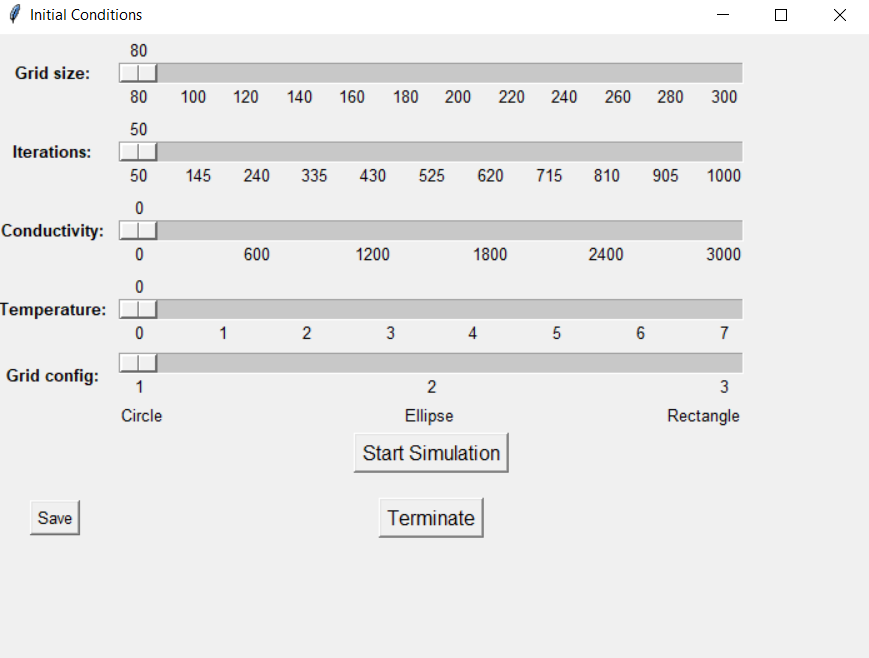
\includegraphics[height=9cm,width=13cm]{images/GUI.png}
    \caption{Input values for the simulation}
    \label{fig:my_GUI}
\end{figure}
Grid size is $l$, iterations or generations is $I$, Conductivity is $c$, Temperature is $T$ within equation \ref{eq1}, and the grid config is what the initial grid looks like at the very first iteration or iteration 0. The user can input one of 3 choices. The "Start" button starts the simulation which will disable all other functionality other than the "Terminate" button which will delete the matplotlib image. The "save" button is meant to save a copy of the animation as a gif file. It is recommended that each action is taken one at a time to avoid unexpected errors. Likewise, the "Terminate" button acts as a reset button which will re-enable all functionality. \par

\vspace{0.3cm}
\noindent
To dynamically change the values of the graph you would need to alter the slider widgets within matplotlib. There are 2 slider widgets within that one of them is a conductivity slide and the other is the temperature slide. You can dynamically change that yourself to the values you desire during the simulation. \par
\begin{figure}[H]
    \centering
    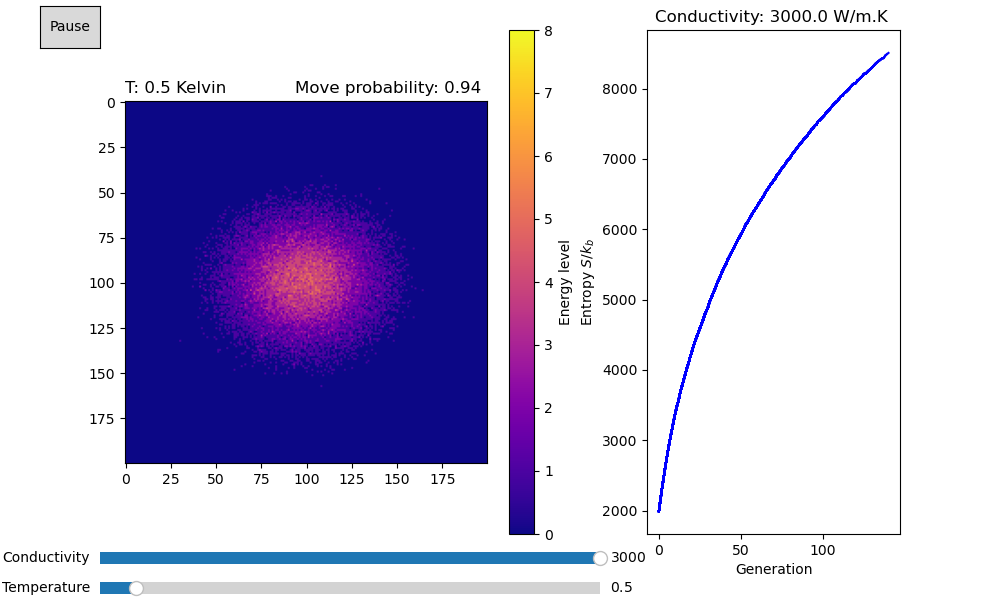
\includegraphics[height=9.5cm,width=15cm]{images/Slider_example.png}
    \caption{Slider widgets within the simulation window}
    \label{fig:dyamic_slide}
\end{figure}
\section{Results}
Now that the GUI system is complete. We could run some analysis by using some standardized initial conditions. For the plots presented below, the length of the grid is $l=100$, the number of iterations is $I=300$, and the grid config is set as "circle". The conductivity and the temperature are made to vary. The results of the simulation are:
\begin{figure}[H]
     \centering
     \begin{subfigure}[h]{0.3\textwidth}
         \centering
         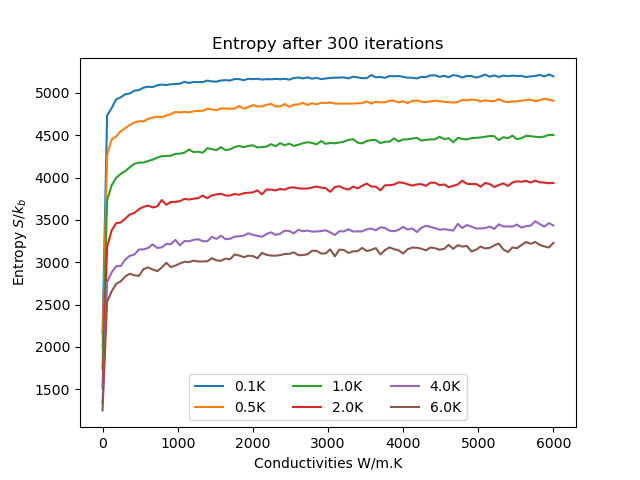
\includegraphics[width=7cm,height=6cm]{images/Entropy_after_300_legend=T.png}
         \caption{Entropy against conductivity}
         \label{fig:directions_1}
     \end{subfigure}
      \hspace{3cm}
     \begin{subfigure}[h]{0.3\textwidth}
         \centering
         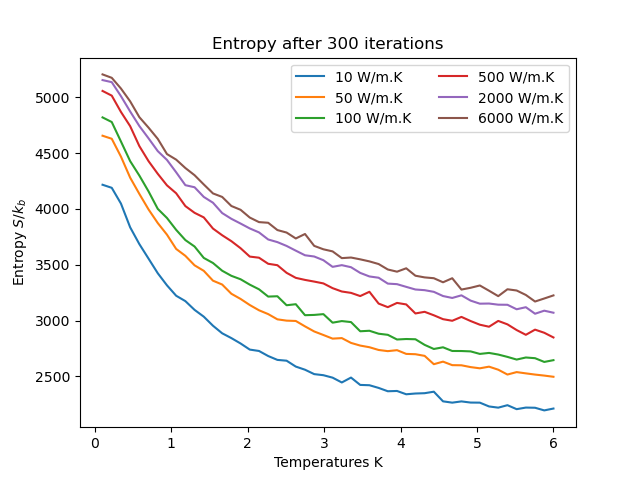
\includegraphics[width=7cm,height=6cm]{images/Entropy_after_300_legend=C.png}
         \caption{Entropy against temperature}
         \label{fig:directions_2}
     \end{subfigure}
        \caption{An explanation of the 2nd law}
        \label{fig:valid_directions}
\end{figure}
As seen from Figure \ref{fig:directions_1}, the final entropy is highly sensitive to changes when conductivity $0<c<500$. This is because of the high growth rate of equation \ref{Mapping} for the first 500 numbers of c. Temperature also plays quite a large role as entropy is decreased when T is greater. Looking at Figure \ref{fig:directions_2}, it is clear that a downward trend exists for increasing temperature levels. Likewise, higher temperature makes the data look more "noisy" with ever-increasing variations for the final entropy measurement. \par

\vspace{0.3cm}
\noindent
While this appears counter-intuitive, there is a very good mathematical explanation of why that is. Looking again at equation \ref{eq1} differences between energy levels are diminished when T is a large big number. Likewise, the omission of the Boltzmann constant $k_{b}$ in calculations exaggerates the effects. As seen from this \href{https://en.wikipedia.org/wiki/Boltzmann_distribution#/media/File:Boltzmann_distribution_graph.svg}{image} in Wikipedia's definition of Boltzmann distribution. The ratios of the probability rapidly approach 1 when T becomes very large.  
$$lim_{T\to\infty} \frac{p_{i}}{p_{j}}=1$$
Reflecting back to equation \ref{eq1}, the exponent term becomes: 
$$lim_{T\to\infty} \frac{8-\epsilon_{j}}{T}=0$$
Therefore, for large values of T, Figure \ref{fig:myfigure2} would look more like: 
\begin{figure}[H]
\centering % center the figure
\begin{tikzpicture}[scale=1.8,minimum size=1.8cm]
    \draw (0,0) grid (3,3);
    \node at (0.5,2.5) [fill=gray!20] {1, \tiny{0.143}} ;
    \node at (1.5,2.5) [fill=gray!20] {3, \tiny{0.143}};
    \node at (2.5,2.5) [fill=gray!20] {2, \tiny{0.143}};
    \node at (0.5,1.5) [fill=gray!20] {7, \tiny{0.143}};
    \node at (1.5,1.5) {6};
    \node at (2.5,1.5) [fill=red!20] {8, \tiny{0}};
    \node at (0.5,0.5) [fill=gray!20] {5, \tiny{0.143}};
    \node at (1.5,0.5) [fill=gray!20] {0, \tiny{0.143}};
     \node at (2.5,0.5) [fill=gray!20] {4, \tiny{0.143}};

    \draw [-stealth] ($(1.5,1.5)!0.4!(0.5,2.5)$) -- ($(1.5,1.5)!0.6!(0.5,2.5)$) ;
    \draw [-stealth] ($(1.5,1.5)!0.4!(1.5,2.5)$) -- ($(1.5,1.5)!0.6!(1.5,2.5)$) ;
    \draw [-stealth] ($(1.5,1.5)!0.4!(2.5,2.5)$) -- ($(1.5,1.5)!0.6!(2.5,2.5)$);
    \draw [-stealth] ($(1.5,1.5)!0.4!(0.5,1.5)$) -- ($(1.5,1.5)!0.6!(0.5,1.5)$) ;
    \draw [-stealth] ($(1.5,1.5)!0.4!(2.5,1.5)$) -- ($(1.5,1.5)!0.6!(2.5,1.5)$) ;
    \draw [-stealth] ($(1.5,1.5)!0.4!(0.5,0.5)$) -- ($(1.5,1.5)!0.6!(0.5,0.5)$) ;
    \draw [-stealth] ($(1.5,1.5)!0.4!(1.5,0.5)$) -- ($(1.5,1.5)!0.6!(1.5,0.5)$) ;
    \draw [-stealth] ($(1.5,1.5)!0.4!(2.5,0.5)$) -- ($(1.5,1.5)!0.6!(2.5,0.5)$) ;

\end{tikzpicture}
\caption{\small {Probabilities of $\frac{1}{7}$ each for the 6 free cells at high T.}}
\label{fig:altered_prob}
\end{figure}
Another interpretation of this is that high temperatures cause a lot of thermodynamic noise, which diminishes the effects of local differences. Now one flaw that my simulation currently has is that it doesn't have a feature that visually tells that the temperature is high. What I might do next is to probably alter the color mapping of matplotlib such that the 0 cells emit more light to display that they are radiating energy. In that case, it's only the differences between cell energy that matter. 